\documentclass{article}

\usepackage[utf8]{inputenc}

\usepackage{natbib}
\usepackage{xcolor}
\usepackage{hyperref}
\hypersetup{
	hidelinks = true,
}

\usepackage{graphicx}

\usepackage[colorinlistoftodos]{todonotes}

\usepackage{parskip}
\setlength{\parskip}{10pt}

\usepackage{tikz}
\usetikzlibrary{arrows, decorations.markings}

% See https://tex.stackexchange.com/questions/425600/latex-error-command-counterwithout-already-defined
\ifdefined\counterwithout\relax\else
  \usepackage{chngcntr}
\fi
\counterwithout{figure}{section}

\begin{document}

\begin{titlepage}


\centering


{\scshape\LARGE Master thesis project \\ planning report\\}

\vspace{0.5cm}

{\huge\bfseries Formally Verified Parser Generator\\}

\vspace{2cm}

{\Large Elias Forsberg (eliasfo@student.chalmers.se)\\}

\vspace{1.0cm}

{\large Supervisor: Andreas Abel\\}

\vfill

{\large \today\\}

\end{titlepage}

\section{Introduction}

	Agda is a functional programming language with a strong type system that
	supports dependent types. Dependent types allow expressing strong invariants and
	properties of data structures and programs, and even constructive proofs
	using the type system. These proofs enable programmers to formally verify
	the correctness of programs and libraries. While the language itself has
	been shown to be sound, neither its parser, nor later stages of its
	compiler have been formally verified. Errors in the implementations of
	these might change the semantics of compiled programs and proofs,
	with severe consequences. % undermining their usefulness.

	Parser generators are commonly used for parsers of programming languages,
	and several different generators exist today, such as Happy~\cite{Happy},
	Bison~\cite{Bison}, and Menhir~\cite{Menhir}. Parser generators are used
\todo{Before using an abbreviation, you have to introduce it.  E.g.:
Backus Naur Form (BNF) descriptions ...

For things like LR(1) or LALR(1) a footnote is more appropriate, as
the unfolding of the abbreviation is long or might need more explanation.
}
	for several reasons: BNF descriptions of grammars are usually more concise
	compared to other representations, such as hand written parsers. Generated
	parsers that are specialized for a language can also be faster compared to
	algorithms that parse any grammar and have to read and analyze the grammar
	of the target language during each parse. Parsers are often required to be
	fast, as they are the first step in what is usually many different passes
	of the entire compilation process. To this end, many parser generators
	generate parsers based on the LR(1) or LALR(1) parsing algorithms. These
	algorithms are designed mainly to be fast, but are unfortunately not able
	to parse all context free grammars.  Other algorithms, such as the Earley
	parsing algorithm~\cite{Earley}, are able to parse all CFG's, while
	maintaining an O(n) time complexity for most unambiguous grammars.

	The BNF Converter~\cite{BNFC} is a parser and lexer generator written in
	Haskell, which uses a labeled BNF description of the target language to
	generate an abstract syntax tree (AST) representation, a parser and a pretty
	printer for the target language. BNFC supports multiple different back-end
	languages (that is, target languages for the generated parser itself), but
	none of these, nor other parts of BNFC have been formally verified. As with
	compilers, errors in parser generators can change the semantics of
	programs, yielding incorrect results.

	% A formally A fverified parser genrator could be used to generate parsers
	% for several A fdifferent formally verified compilers

	% Nice if BNFC was guarantied to generate correct parsers.

	Verified compilers have received significant attention in the research
	community. CompCert~\cite{Leroy} is a formally verified compiler for a
	subset of the C programming language. It is written in Coq, a proof assistant similar to
	Agda, and is accompanied by Coq-proofs that it preserves
	the semantics of compiled programs.
	This compiler does not, however, do any form of verification of the
	parsing step, but starts from the AST level. If verified parsers could be
	easily generated for use in different programming languages, it would be
	possible to have compilers that are fully verified from source code in its
	original text format to the output of the compiler.

	The aim of this thesis is to create a parser generator that can create a
	parser for any context-free grammar, using (possibly among others) the
	Earley parsing algorithm, and to formally verify, using Agda, that all
	generated parsers are correct\footnote{\emph{Correct} meaning sound and complete.}.

	% This parser generator could then potentially be used to generate a parser
	% for Agda.

\section{Context}

	Research in formal verification and parsing has been done previously by
	several groups. Below we discuss some research related to this project.

	Jourdan and Pottier~\cite{Jourdan} demonstrated
\todo{Scientific results should be cited in present tense in
  general, as these are eternal truths (or at least intended
  to be such):  J and P demonstrate...}
	a method for verifying the
	correctness of generated LR parsers. They used the fact that LR parsers are
	stack automata guided by a finite-state automaton, and designed a verifier
	that can check whether a given automaton conforms to a specified grammar.
	As such, they did not prove the correctness of the parser generator itself.
	Further, their method does not verify parsers capable of parsing any context-free
	grammar.

	Firsov and Uustalu~\cite{Firsov14} verified a CYK parsing algorithm using
	Agda. The CYK parsing algorithm only works for grammars in Chomsky normal
	form, which is not the natural representation of the grammars
	for most target languages. This
	means that the grammar will first have to be normalized, a process which
	also should be verified in order to have a fully verified parsing process.
	Fortunately, Firsov and Uustalu later verified a normalization algorithm
	for context free grammars.~\cite{Firsov15} The normalization process can,
	however, increase the size of the grammar, up to a quadratic increase. This
	might be undesirable for some situations where very large grammars are
	used.

	Ridge~\cite{ridge11} verified a parser generator for context-free grammars
	that is both sound and (mostly) complete. However, while it is able to
	parse all CFG's, it is not able to produce all syntax tree derivations for
	some ambiguous grammars. Further, generated parsers have a time complexity
	of O($n^5$), which is significantly worse than the O($n^3$) time
	complexity of, e.g., CYK. This can be undesirable for some applications.

	While these works are closely related, this thesis will aim to verify a
	parser generator for all context-free grammars. This means that a parser
	will be created for each target grammar, and ideally that this parser could
	be emitted in several different target languages. The thesis will also use
	the Earley parsing algorithm, which has not previously been formally
	verified.

\section{Goals and Challenges}

	% This section currently includes
	% - Aim for the work. What should be accomplished?
	% - The formulation of the problem at hand and, the assignment. This should
	%   include an extended version of the scientific problem definition and
	%   references to knowledge within the area given in the thesis proposal.

	This thesis will aim to verify a parser generator for context-free
	grammars. A useful parser generator should most likely include an easy to
	use method for defining and reading the definitions of grammars, as well as
	generation of both parsers and lexers\footnote{While a lexer might not be
	strictly necessary to parse context-free grammars given a complete parser,
	defining a tokenization step before parsing can be useful for implementers.
	Lexers can also be faster in some circumstances}. A parser generator will
	also be significantly more useful if it is able to generate parsers in
	several different back-end languages, as this will make it easier to use
	the generator for many different projects.  Steps toward a formally
	verified parser generator might look something like:

	\begin{enumerate}

		\item \label{lex}

			Implement a lexer, and prove its correctness.

		\item \label{par}

			Implement a parser, and prove its correctness.

		\item \label{lbnf}

			Design a syntax for grammar definitions and use the parser from
			step \ref{par} to parse it.

		\item \label{dsl}

			Design an intermediate representation for generated lexers and
			parsers.

		\item \label{lexgen}

			Implement a lexer generator, prove its correctness.

		\item \label{pargen}

			Implement a parser generator, and prove  its correctness.

		\item \label{backend}

			Implement a compiler from the intermediate representation to some
			back-end language, such as Agda or C, and prove its correctness.

	\end{enumerate}

	\subsection{Limitations}

%		Everything else: grammar definition files, lexer, lexer generator,
%		backend, no user interface. But reserving the right to extend project,
%		should the time be sufficient.

		This project will mainly focus on parsing of context free grammars, and
		as such neither the lexer (step \ref{lex}) nor the lexer generator
		(step \ref{lexgen}) will be a priority. It is also hard to estimate how
		long steps \ref{dsl}-\ref{backend} will take. Concluding after only
		completing steps \ref{par} and \ref{lbnf} will be sufficient for
		completing the project, if correctness proofs of the implemented parser
		are complete.  Steps \ref{lbnf} and \ref{pargen} have room for many
		optimizations and user experience improvements, but any of these would
		be optional. While step \ref{backend} would be necessary for a
		end-to-end verified compiler, it might be a very large task, depending
		on the target language.

		Because of reasons mentioned above, this project will most likely
		conclude without steps \ref{lex}, \ref{lexgen}, and \ref{backend}.

	\subsection{Problem Formulation}

		The main goals of this project are: firstly, to create and formally
		verify the correctness of an Earley parser, and secondly, to create and
		formally verify the correctness of a parser generator for context-free
		grammars.


\section{Approach}
	% - Method of accomplishment. How should the work be carried out?

	Creating the initial parser (step \ref{par} above) will be useful for
	parsing the grammar syntax files in order to read the definitions of the
	parsers that should be generated. This initial proof of a parser is also
	expected to be simpler than the full generator proof, and might severe as
	guiding steps for the full proof.

	The grammar syntax files (step \ref{lbnf} above) will use BNFC's
	Labeled BNF format, and these will also be used to generate the AST
	representation. If possible, we hope to maintain compatibility with BNFC,
	as several existing projects would then be able to have their parsing
	formally verified without modifications.

	The intermediate representation for parsers and lexers (step \ref{dsl}
	above) will ideally be designed with simple semantics. The semantics of
	this language could be defined using an interpreter written in Agda. This
	will help disconnect the correctness proof of the parser generator from the
	semantics of any potential target languages, as these may be quite complex.
	We hope that this will lighten the proof burden for the parser generator.

	% Lexer generator and parser generator proofs the real meat of this
	% project.

	The final step of the parser generator, compiling the intermediate
	representation to the target parser language (step \ref{backend} above),
	while necessary for a complete end-to-end verified parser, is potentially a
	lot of work to verify. The semantics of each target language would first
	have to be formalized, if they are not already, and it would then be
	necessary to prove that the compiler preserves the semantics of the
	intermediate representation under this formalization. An \emph{un}verified
	compiler for the intermediate representation might be constructed for this
	project, so that the parser generator can be used even if all steps have
	not been verified.

	% Proofs themselves can't be tested/evaluated?  Compare speed to LR and
	% LALR parsers?

\section{Ethical Considerations}

	As with any tool, a parser generator could be used for many different
	purposes, but a parser generator itself is unlikely to cause harm. There
	are also no significant risks, except for loss of time spent, of conducting
	the work, and the project does not have any stakeholders external to
	Chalmers University of Technology.

\section{Time Plan}

	Below is a preliminary time plan for this project:

	\begin{figure}
		\centering
		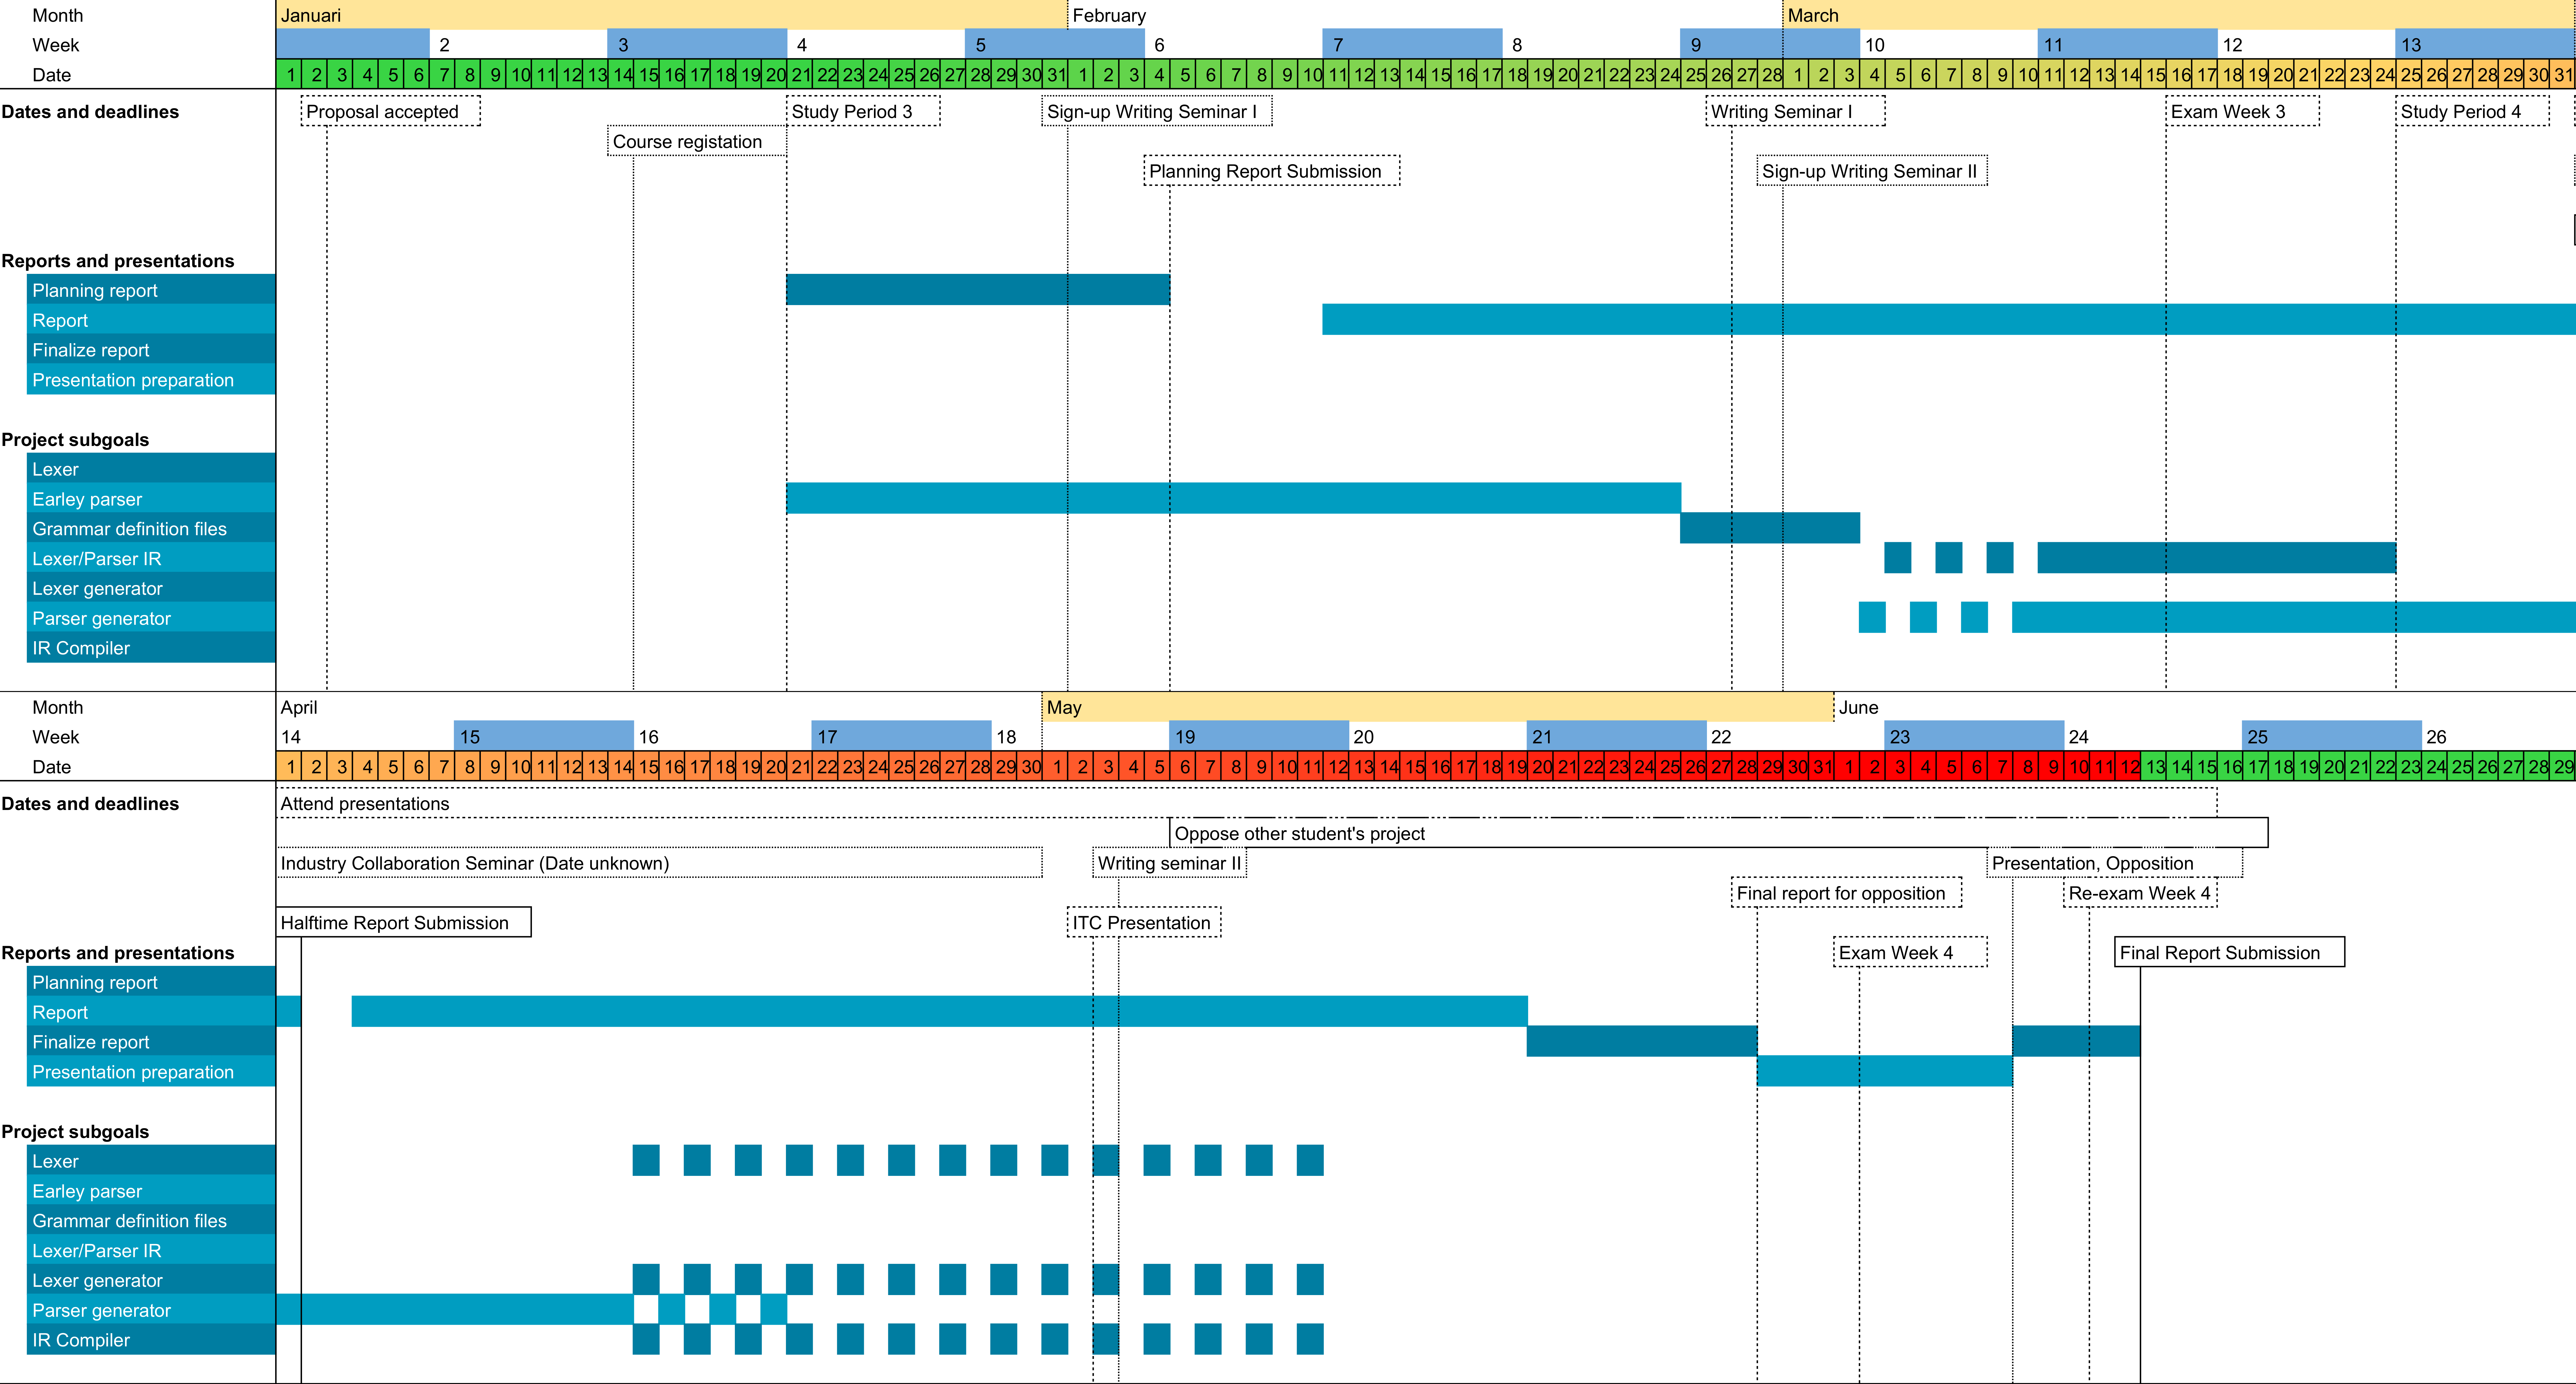
\includegraphics[angle=-90,width=0.75\textwidth]{gantt.png}
	\end{figure}

\newpage

\bibliographystyle{plain}

\bibliography{lit}

\end{document}
